%-------------------------------------------------------------------------------
%-------------------------------------------------------------------------------
%-------------------------------------------------------------------------------
\chapter{Bases de données}
%-------------------------------------------------------------------------------
%-------------------------------------------------------------------------------
\thispagestyle{empty}
%-------------------------------------------------------------------------------
%-------------------------------------------------------------------------------
\section{Présentation}
%--------------------------------------------------------------------------
%--------------------------------------------------------------------------
Notre société utilise de plus en plus de données et un des enjeux de l'efficacité économique mais aussi de la démocratie est d'en maîtriser l'exploitation.

Nous allons décrire dans ce chapitre le modèle de description d'un ensemble de données, les opérations qu'on veut pouvoir effectuer et le langage universel qui permet ces opérations.
%--------------------------------------------------------------------------
%--------------------------------------------------------------------------
\subsection{Données}
%--------------------------------------------------------------------------
%--------------------------------------------------------------------------
Un ensemble de données est avant tout constitué d'information, l'enjeu est d'arriver à trouver une réponse depuis ces ensemble d'information. Quand les données ne sont pas bien structurées cela peut devenir une énigme, comme dans certains jeux.

%--------------------------------------------------------------------------
\begin{minipage}{0.7\linewidth}
{\it Le dahut est une espèce très rare de bouquetin qui a la particularité d'avoir les deux pattes d'un coté plus courtes que les autres. Il vit donc dans la montagne en ayant toujours le sommet du coté de ses pattes courtes. Un dahut est appelé de dextrogyre (resp. lévogyre) si ses pattes gauches (resp. ses pattes droites) sont plus courtes, ce qui fait qu'il a le sommet de sa montagne sur sa droite (resp. sur sa gauche) et que donc il tourne toujours vers la droite (resp. vers la gauche).

Les dahuts ont d'autres particularités :
 
\begin{itemize}
\item tout dahut non lévogyre a des rayures noires,
\item tout dahut a des oreilles blanches ou n'a pas de rayures noires,
\item les dahuts qui vivent dans les forêts ne mangent pas de mulots,
\item un  dahut mange des mulots si et seulement s'il est lévogyre,
\item tout dahut qui a des oreilles blanches est lévogyre et vit dans les forêts,
\item tout dahut lévogyre a des oreilles blanches.
\end{itemize}

Prouver que les dahuts n'existent pas.}
\end{minipage}
\begin{minipage}{0.25\linewidth}
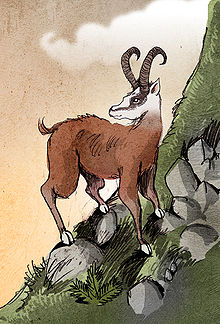
\includegraphics[width=4cm]{17_dahut}
\end{minipage}
%---------------------------------------------------------

\medskip

Pour organiser les données on va utiliser un modèle simple, celui d'un tableau.

Les données concernent plusieurs objets qui ont des propriétés, on se donne à l'avance un ensemble de caractéristiques et on donne, pour chaque objet, la valeur prise pour chaque caractéristique. On obtient un tableau à deux dimensions avec une ligne par objet et une colonne par caractéristique. Les colonnes sont nommées mais les objets sont définis simplement par leur ensemble de valeurs, s'ils ont un nom alors c'est une de leurs propriétés.

\newpage

On rencontre souvent ce type de structures :
%--------------------------------------------------------------------------
\begin{itemize}
\item répertoire (nom, téléphone, adresse, ...)
\item fiche de bibliothèque (auteur, titre, année, pagination, ...)
\item livre d'état-civil des naissances (père, mère, nom, lieu, ...)
\item ...
\end{itemize}
%--------------------------------------------------------------------------

Voici un exemple simple dont nous nous servirons. Ce sont les vainqueurs des élections présidentielles de la cinquième république.
%--------------------------------------------------------------------------
\begin{center}
\begin{tabular}{|c|c|c|c|c|c|c|}
\hline
{\bf nom} &{\bf prénom} & {\bf études}& {\bf politique}& {\bf année}&{\bf résultat}\\
  \hline
de Gaulle & Charles & Saint-Cyr&D& 1958&78,5\\
de Gaulle & Charles & Saint-Cyr&D&1964&55,2\\
Pompidou & Georges & ENS Ulm&D& 1969&58,2\\
Giscard d'Estaing &Valery&X&C&1974&50,8\\
Miterrand &François&Droit&G&1981&51,8\\
Miterrand &François&Droit&G&1988&54,0\\
Chirac &Jacques&ENA&D&1995&52,6\\
Chirac &Jacques&ENA&D&2002&82,2\\
Sarkozy &Nicolas&Droit&D&2007&53,0\\
Hollande &François&ENA&G&2012&51,6\\
Macron &Emmanuel&ENA&C&2017&66,1\\
\hline
\end{tabular}
\end{center}
%--------------------------------------------------------------------------
%--------------------------------------------------------------------------
\subsection{Travailler sur des données}
%--------------------------------------------------------------------------
%--------------------------------------------------------------------------
\subsubsection{Travail en direct}
%--------------------------------------------------------------------------
La première possibilité pour traiter ces données, et qui reste certainement la plus courante, est d'utiliser un {\sc tableur}. C'est une solution très simple qui permet de faire des calculs sur des données quand on n'a pas besoin d'en extraire une partie. On peut trier selon une caractéristique, faire des calculs globaux (statistiques), faire des combinaisons de valeurs mais il est difficile de faire des moyennes partielles, par exemple dans le tableau ci-dessus, calculer la moyenne des résultats par couleur politique.

De plus il est difficile de permettre l'utilisation par plusieurs personnes d'une même base.
%--------------------------------------------------------------------------
\subsubsection{L'architecture client-serveur}
%--------------------------------------------------------------------------
On a choisi d'abstraire la base de données en la plaçant sur un {\sc serveur}, chaque utilisateur, ou {\sc client}, envoie ses demandes, on parle de {\sc requêtes}, au serveur qui lui répond. 

%--------------------------------------------------------------------------
\begin{center}
\tikzpicture
\node[circle, draw, minimum size =15mm] (c1) at (0,0) {Client 1};
\node[circle, draw, minimum size =15mm] (c2) at (7, 2) {Client 2};
\node[circle, draw, minimum size =15mm] (c3) at (9,-2) {Client 3};
\node[circle, draw, minimum size =15mm] (c4) at (2,-4) {Client 4};
\node[draw, minimum size =15mm] (s) at (4,0) {Serveur};
\draw[stealth-stealth] (c1)--(s) ;
\draw[stealth-stealth] (c2)--(s) ;
\draw[stealth-stealth] (c3)--(s) ;
\draw[stealth-stealth] (c4)--(s) ;
\endtikzpicture
\end{center}
%--------------------------------------------------------------------------



Il ne faut pas se fier à la simplicité apparente de cette structure, les problèmes à gérer sont nombreux et délicats :
\begin{itemize}
\item organisation des données,
\item rapidité d'accès,
\item gestion des autorisations d'accès,
\item priorités des accès,
\item sauvegarde des modifications,
\item gestion des pannes ...
\end{itemize}

Il faut donc un langage pour établir les requêtes auprès d'un serveur. Ici, un phénomène inhabituel en informatique s'est produit, 
Cependant, contrairement aux langages de programmation, un standard a été choisi, c'est le langage SQL que nous allons partiellement exposer dans la suite. Ce langage permet de définir, modifier, interroger les différents systèmes du point de vue des utilisateurs. Bien entendu la programmation en interne de ces gros logiciels dépend de l'éditeur (Oracle, SAP, IBM, Microsoft, ...) 



%--------------------------------------------------------------------------
\subsubsection{Pour les utilisateurs}
%--------------------------------------------------------------------------
On peut remarquer que SQL n'est pas visible pour les usagers. 
En effet l'utilisation des bases de données se fait maintenant à travers une architecture {\sc trois-tiers}. Entre l'usager et la base de données se place l'application qui travaille au dessus du gestionnaire de bases de données.
%--------------------------------------------------------------------------
\begin{center}
\tikzpicture[scale=0.8]
\node[draw,circle,minimum size =18mm] (c1) at (-2,0) {Client};
\node[draw,circle,,minimum size =18mm] (c2) at (1,4) {Client};
\node[draw,circle,minimum size =18mm] (c3) at (1,-4) {Client};
\node[draw,circle,minimum size =24mm] (a) at (4,0) {Application};
\node[draw,circle,minimum size =24mm] (s) at (9,0) {Serveur};
\draw[stealth-stealth] (c1)-- node[above]{interface html}(a) ;
\draw[stealth-stealth] (c2)-- (a) ;
\draw[stealth-stealth] (c3)-- (a) ;
\draw[stealth-stealth] (a)-- node[below]{SQL}(s) ;
\endtikzpicture
\end{center}
%--------------------------------------------------------------------------
\subsubsection{Plan}
%--------------------------------------------------------------------------
Dans la suite nous allons d'abord présenter le modèle des tableaux et le vocabulaire associé, puis nous définirons les opérations souhaitées. La partie suivante donnera la traduction opératoire de ces concepts dans le langage SQL.

On introduit enfin les outils statistiques.

Le chapitre suivant exposera un autre aspect de ce modèle, la possibilité de croiser plusieurs tables de données.
%--------------------------------------------------------------------------
\newpage
%--------------------------------------------------------------------------
%--------------------------------------------------------------------------
\section{Relations}
%--------------------------------------------------------------------------
\subsection{Vocabulaire}
%--------------------------------------------------------------------------
La composante de base, le tableau, est appelé {\bf relation}.

On a vu qu'il comportait deux parties :
%--------------------------------------------------------------------------
\begin{itemize}
\item les différents titres des colonnes qui sont appelés {\bf attributs} ; on appelle {\bf schéma} ({\bf sort} en anglais) l'ensemble des attributs,

\item l'ensemble des lignes est l'{\bf extension} de la retaion, une ligne sera nommée {\bf n-uplet} ({\bf tuple} en anglais).
\end{itemize}
%--------------------------------------------------------------------------

On nommera $A_1,A_2,\ldots,A_p$ les attributs.

L'ensemble des valeurs possibles d'un attribut $A$ est son domaine Dom($A$).

Chaque  n-uplet est donc un élément de $\text{Dom}(A_1)\times \text{Dom}(A_2)\times \cdots \times \text{Dom}(A_p)$.
%--------------------------------------------------------------------------
\subsection{Contraintes}
%--------------------------------------------------------------------------
La définition énoncée ci-dessus implique des contraintes. Certaines de ces conséquences devront être assurées par l'utilisateur d'autres seront contrôlées par le logiciel.
%--------------------------------------------------------------------------
\subsubsection{Les attributs forment un ensemble}
%--------------------------------------------------------------------------
\begin{itemize}
\item Il n'y a pas d'attribut en double : il ne peut être question qu'il y ait deux attributs de même nom, ils risqueraient d'être affectés de valeurs différentes dans des n-uplets.
%--------------------------------------------------------------------------
\item L'ordre des attributs n'est pas fixé : 

on ne parle pas du premier attribut mais de l'attribut {\tt nom\_attribut} (par exemple).
%--------------------------------------------------------------------------
\item En conséquences les différentes données ne sont donc pas des n-uplets au sens informatique du terme. Ce sont plutôt des fonctions depuis l'ensemble des attributs vers l'union des domaines avec la condition que $t[A_i]$ appartient au domaine $\text{Dom}(A_i)$ (remarquer que l'on écrit avec des crochets plutôt que des parenthèses).
%--------------------------------------------------------------------------
\item On peut alors restreindre une ligne à un sous-ensemble d'attributs : si $S$ est une partie de $\{A_1,A_2,\ldots,A_p\}$ on notera $t[S]$ l'ensemble des valeurs prises par le n-uplet $t$ pour les attributs appartenant à $S$, par exemple 
$t[A_4,A_5,A_2]$.
\end{itemize}
%--------------------------------------------------------------------------
\subsubsection{Les lignes forment un ensemble}
%--------------------------------------------------------------------------
\begin{itemize}
\item Il n'y a pas de ligne en double : si $t[A_1,\ldots,A_p]=t'[A_1,\ldots,A_p]$ alors $t=t'$ ; cela correspond à l'aspect fonction des n-uplets.
%--------------------------------------------------------------------------
\item L'ordre des lignes n'est pas fixé.
\end{itemize}
%--------------------------------------------------------------------------

\medskip


Bien entendu une présentation des données dans un tableau aura un ordre des attributs et un ordre des n-uplets mais ces ordres de présentations sont le résultats des choix de l'utilisateur ou de l'ordre physique des données.

\newpage
%--------------------------------------------------------------------------
\subsection{Clés}
%--------------------------------------------------------------------------
La contrainte de non-répétition des n-uplets est très importante ; la répétition de données induirait des problème de rapidité d'accès et fausserait les calculs. Pour cela les bases de données réelles contiennent un concept de {\bf clé} qui doit être pensé dès la conception des bases de données. On verra qu'il a aussi une grande importance lors de l'utilisation de relations multiples.
%--------------------------------------------------------------------------
\begin{defin}[Super-clé]

Une super-clé d'une relation $r$ est un ensemble $S$ d'attributs tel que
\[\forall t,t' \in R\quad \bigl(t[S]=t'[S]\bigr) \Rightarrow (t=t')\]
\end{defin}
%--------------------------------------------------------------------------
Les contraintes imposent que l'ensemble de tous les attributs est toujours une super-clé.

\medskip

Dans l'exemple ci-dessus $\{\texttt{année}\}$, 
$\{\texttt{nom},\texttt{résultat}\}$, 
$\{\texttt{prénom},\texttt{année}\}$ sont des super-clés.

%--------------------------------------------------------------------------
\begin{defin}[Clé candidate]

Une clé candidate d'une relation $r$ est une super-clé minimale pour l'inclusion.
\end{defin}
%--------------------------------------------------------------------------

$K$ est donc une clé candidate si
%--------------------------------------------------------------------------
\begin{enumerate}
\item $K$ est une super-clé
%--------------------------------------------------------------------------
\item Pour tout $K'$ inclus dans $K$, $K'$ n'est pas une super-clé.
\end{enumerate}
%--------------------------------------------------------------------------
Une super-clé qui ne contient qu'un seul attribut est toujours une clé candidate.
%--------------------------------------------------------------------------
\begin{itemize}
\item $\{\texttt{nom},\texttt{résultat}\}$ n'est pas une clé candidate. 
%--------------------------------------------------------------------------
\item $\{\texttt{année}\}$ est une clé candidate. 
%--------------------------------------------------------------------------
\item Lorsque vous vous identifiez sur un site sur lequel vous êtes inscrit, 

l'identifiant + le mot de passe est une clé candidate.
\end{itemize}
%--------------------------------------------------------------------------
\begin{defin}[Clé primaire]

Parmi les clés candidates on en choisit une : c'est la clé primaire.
\end{defin}
%--------------------------------------------------------------------------
Pour indiquer la clé primaire on souligne les attributs correspondants dans la table.

Indiquer au système une clé primaire pour chaque table permet une indexation des données à l'aide
de cette clé, ce qui renforce l'efficacité des procédures d'interrogation de la table.

Nous connaissons déjà ce genre d'attributs : 

numéro de sécurité sociale, plaque minéralogique, numéro de série \dots

Pour obtenir une clé primaire efficace il est recommandé introduire un attribut, souvent nommé {\tt id}, dans la définition de la relation. 

Ce sera un entier qu'on incrémentera à chaque ajout d'un n-uplet.
%--------------------------------------------------------------------------
\begin{center}
\begin{tabular}{|c|c|c|c|c|c|c|}
\hline
{\bf \underbar{id}}&{\bf nom} &{\bf prénom} & {\bf études}& {\bf politique}& {\bf année}&{\bf résultat}\\
  \hline
1&de Gaulle & Charles & Saint-Cyr&D& 1958&78,5\\
2&de Gaulle & Charles & Saint-Cyr&D&1964&55,2\\
3&Pompidou & Georges & ENS Ulm&D& 1969&58,2\\
4&Giscard d'Estaing &Valery&X&C&1974&50,8\\
5&Miterrand &François&Droit&G&1981&51,8\\
6&Miterrand &François&Droit&G&1988&54,0\\
7&Chirac &Jacques&ENA&D&1995&52,6\\
8&Chirac &Jacques&ENA&D&2002&82,2\\
9&Sarkozy &Nicolas&Droit&D&2007&53,0\\
10&Hollande &François&ENA&G&2012&51,6\\
11&Macron &Emmanuel&ENA&C&2017&66,1\\
\hline
\end{tabular}
\end{center}
%--------------------------------------------------------------------------
\newpage
%--------------------------------------------------------------------------
\section{Algèbre relationnelle simple}
%--------------------------------------------------------------------------
%--------------------------------------------------------------------------
Pour modéliser les requêtes on va considérer qu'une relation n'est qu'une relation parmi toutes les relations possibles et on a va modéliser la construction de relations à partir d'autres relations.

Depuis 1970 deux modèles abstraits de structure des données et d'extraction ont été étudiés : l'algèbre relationnelle et le calcul relationnel. 

L'{\bf algèbre relationnelle} formalise les opérations qui doivent être faites, le {\bf calcul relationnel} décrit ce que l'on veut obtenir.

Ces deux modèles sont équivalents et ont servi de base théorique aux logiciels de base de données que les progrès de l'informatique ont permis d'écrire de manière efficace. 

Nous allons étudier l'un de ces modèles : l'algèbre relationnelle.
%--------------------------------------------------------------------------
\subsection{Définition}
%--------------------------------------------------------------------------
L'algèbre relationnelle est un ensemble d'opérateurs que l'on peut appliquer à des relations, et dont le résultat est une relation.

Comme le résultat est toujours une relation on pourra combiner ces opérateurs : on forme ainsi des {\bf requêtes} élaborées.

L'objectif est de pouvoir exprimer toute requête raisonnable par une combinaison d'opérateurs élémentaires.

{\bf Exemples de requêtes} sur le tableau donné en exemple.
%--------------------------------------------------------------------------
\begin{itemize}
\item Quels sont les présidents de droite ?
%--------------------------------------------------------------------------
\item Quels sont les présidents qui sortent de l'ENA ?
%--------------------------------------------------------------------------
\item Quels présidents ont gouverné plus de 10 ans ?
\end{itemize}
%--------------------------------------------------------------------------
\subsection{Opérateurs ensemblistes}
%--------------------------------------------------------------------------
Un premier type d'opérateur combine 2 relations qui ont le même schéma ; on les utilisera surtout pour assembler les résultats d'autres requêtes.

$r$ et $r'$ sont deux relations ayant le même schéma (c'est-à-dire les mêmes attributs).
%--------------------------------------------------------------------------
\begin{enumerate}
\item $r \cup r'$ est la relation de même schéma dont les n-uplets appartiennent à $r$ {\bf ou} à $r'$.
%--------------------------------------------------------------------------
\item $r \cap r'$ est la relation de même schéma dont les n-uplets appartiennent à $r$ {\bf et} à $r'$.
%--------------------------------------------------------------------------
\item $r \setminus r'$ est la relation de même schéma dont les n-uplets  appartiennent à $r$ {\bf mais pas} à $r'$.
\end{enumerate}
%--------------------------------------------------------------------------
\subsection{Opérateurs spécifiques}
%--------------------------------------------------------------------------
Les opérateurs étudiés ici sont ceux qui utilisent la structure des relations. Dans cette partie nous n'étudions que les opérateurs unaires, qui s'appliquent à une relation unique.

Par exemple la question ``Quels sont les présidents qui sortent de l'ENA ?'' se traduit par :

donner les noms (projection) des présidents dont les études se sont passées à l'ENA (sélection).

\medskip

Le {\bf RENOMMAGE} consiste à renommer un attribut. 

Ce sera utile lors de produits de tables lorsque deux tables ont des attributs portant le même nom mais correspondent à des données différentes.

Si $A\in R$ où $R$ est le schéma de $r$ et $B\not\in R$ on note $\rho_{A \rightarrow B}(r)$ la relation obtenue en changeant le nom de l'attribut $A$ en $B$. 
%--------------------------------------------------------------------------
\begin{enumerate}
\item Si $R$ est le schéma de $r$ avec $A\in R$, le schéma de $\rho_{A \rightarrow B}(r)$ est $(R\setminus\{A\})\cup\{B\}$.
%--------------------------------------------------------------------------
\item L'extension de $\rho_{A \rightarrow B}(r)$ est $\bigl\{t\ ;\   \exists s\in r, t[B]=s[A], \forall C\in R\setminus\{A\},\  t [ C ]=s [C ]\bigr\}$.
\end{enumerate}
%--------------------------------------------------------------------------
\medskip

La {\bf SELECTION} (ou restriction) consiste à ne garder que les n-uplets qui vérifie une propriété. 

On note $\sigma_F(r)$ la relation extraite de $r$ par la propriété $F$.
%--------------------------------------------------------------------------
\begin{enumerate}
\item $\sigma_F(r)$ a le même schéma que $r$
%--------------------------------------------------------------------------
\item L'extension de $\sigma_F(r)$ est $\bigl\{t\in r\ ;\  t\hbox{ vérifie }F\bigr\}$
\end{enumerate}
%--------------------------------------------------------------------------
On notera, pas abus d'écriture, $\sigma_F(r)=\bigl\{t\in r\ ;\  t\hbox{ vérifie }F\bigr\}$ sans noter explicitement le schéma.

\medskip

Les propriétés élémentaires sont de la forme $P\, \theta\,Q$ 

où $\theta$ un opérateur de comparaison ($=$, $<$, $\le$, $>$, $\ge$) et $P$ et $Q$ des expression construites à partir des attributs et des constantes avec des fonctions usuelles.

\medskip

Une propriété composée avec des connecteurs logiques correspond à des unions et intersections et peut être écrite directement. 

Par exemple $\sigma_{F\,et\,F'}(r)=\sigma_{F}(r) \cup \sigma_{F'}(r)$.

\medskip

{\bf Exemple} :  $F$ est la condition ``prénom = François'', $\sigma_F(r)$ est la relation
%--------------------------------------------------------------------------
\begin{center}
\begin{tabular}{|c|c|c|c|c|c|c|}
\hline
{\bf \underbar{id}}&{\bf nom} &{\bf prénom} & {\bf études}& {\bf politique}& {\bf année}&{\bf résultat}\\
  \hline
5&Miterrand &François&Droit&G&1981&51,80\\
6&Miterrand &François&Droit&G&1988&54,0\\
10&Hollande &François&ENA&G&2012&51,6\\
  \hline
\end{tabular}
\end{center}

\medskip

La {\bf PROJECTION} consiste à ne garder qu'une partie des attributs. On note
$\pi_X(r)$ la relation extraite de $r$ avec les restriction des n-uplets à l'ensemble $X$.
%--------------------------------------------------------------------------
\begin{enumerate}
\item $\pi_X(r)$ admet $X$ pour schéma.
%--------------------------------------------------------------------------
\item L'extension de $\pi_X(r)$ est $\bigl\{t[X] ;\  t\in r\bigr\}$
\end{enumerate}
%--------------------------------------------------------------------------
On notera, pas abus d'écriture, $\pi_X(r)=\bigl\{t[X] ;\  t\in r\bigr\}$ sans noter explicitement le schéma et en assimilant la restriction à $X$ avec l'image $t[X]$.

{\bf Exemple} : si $X$ est l'ensemble \{prénom, nom, résultat\}, 
$\pi_X(r)$ est la relation
%--------------------------------------------------------------------------
\begin{center}
\begin{tabular}{|c|c|c|c|c|c|c|}
\hline
{\bf nom} &{\bf prénom} &{\bf résultat}\\
  \hline
de Gaulle & Charles &78,5\\
de Gaulle & Charles &55,2\\
Pompidou & Georges &58,2\\
Giscard d'Estaing &Valery&50,8\\
Miterrand &François&51,8\\
Miterrand &François&54,0\\
Chirac &Jacques&52,6\\
Chirac &Jacques&82,2\\
Sarkozy &Nicolas&53,0\\
Hollande &François&51,6\\
Macron &Emmanuel&66,1\\
\hline
\end{tabular}
\end{center}
%--------------------------------------------------------------------------
Comme la projection doit être une relation les lignes ne sont pas répétées : 

si $X$=\{étude\}, $\pi_X(r)$ donne
%--------------------------------------------------------------------------
\begin{center}
\begin{tabular}{|c|}
\hline
{\bf études}\\
  \hline
Saint-Cyr\\
  \hline
 ENS Ulm\\
  \hline
Polytechnique\\
  \hline
Fac de droit\\
  \hline
ENA\\
  \hline
\end{tabular}
\end{center}
%--------------------------------------------------------------------------
\newpage
%--------------------------------------------------------------------------
\section{SQL}
%--------------------------------------------------------------------------
%--------------------------------------------------------------------------
\subsection{Introduction}
%--------------------------------------------------------------------------
Nous venons de décrire les premiers opérateurs de l'algèbre relationnelle. 

On peut les comparer aux instructions de bases en programmation. 

Pour les langages de requêtes il s'est produit un événement inhabituel : une norme universelle a été établie qui permet d'écrire des requêtes de la même façon quel que soit le logiciel : c'est {\bf SQL}, pour {\sc Structured Query Langage}.

Le langage SQL reprend la structure de l'algèbre relationnelle en y ajoutant des moyens de calculs et autres améliorations. Il le fait dans une formulation plus proche d'un langage humain (l'anglais) en structurant les requêtes dans un modèle simple.

Bien entendu chaque éditeur optimise les opérateurs pour donner des réponses le plus rapidement possible, ajoute des améliorations supplémentaires mais presque tous contiennent le langage tel qu'il est normalisé.

\medskip
%--------------------------------------------------------------------------
\subsection{Instructions de base}
%--------------------------------------------------------------------------
Les représentations des relations se font avec le modèle du tableau.

En SQL on parlera de 
%--------------------------------------------------------------------------
\begin{itemize}
\item {\bf tables} à la places de relations
%--------------------------------------------------------------------------
\item {\bf colonnes} à la places d'attributs
%--------------------------------------------------------------------------
\item {\bf lignes} à la places de n-uplets.
\end{itemize}
%--------------------------------------------------------------------------
La forme de base d'une requête en SQL est une composition d'une sélection et d'une projection.
%--------------------------------------------------------------------------
\begin{lstlisting}[language=SQL]
FROM table1
WHERE condition;
\end{lstlisting}
%--------------------------------------------------------------------------
Les mots-clés de SQL sont usuellement écrits en majuscule mais ce n'est pas obligatoire
%--------------------------------------------------------------------------
\begin{description}
\item[SELECT] correspond à la projection, les attributs ou colonnes à afficher sont énumérés et séparés par une virgule. Il y a toujours une projection.

Si on ne veut pas effectuer de projection, on doit indiquer que l'on veut toutes les colonnes. On peut le faire par le symbole * qui signifie "tout".
%--------------------------------------------------------------------------
\item[FROM] sélectionne le nom de la table à utiliser. 

Cela deviendra plus signifiant lorsqu'on utilise plusieurs tables.
%--------------------------------------------------------------------------
\item[WHERE] correspond à la sélection (attention : \type{SELECT} ne désigne pas la sélection ). 

La condition peut être composée à l'aide des connecteurs logiques \type{AND}, \type{OR} ou \type{NOT}. 

Les comparateurs sont \type{=}, \type{>}, \type{<}, \type{>=}, \type{<=}, \type{!=}. 

Les chaînes de caractères sont entourées de guillemets simples ou doubles.

La clause \type{WHERE} est facultative. On peut ne pas faire de sélection.
%--------------------------------------------------------------------------
\item[AS] On peut renommer une colonne avec {AS} suivi du nouveau nom.
%--------------------------------------------------------------------------
\item[UNION, INTERSECT, EXCEPT] Si on veut combiner plusieurs requêtes on peut les assembler avec \type{UNION} (pour $\cup$), \type{INTERSECT} (pour $\cap$) ou \type{EXCEPT} (pour $\setminus$).
\end{description}
%--------------------------------------------------------------------------

\medskip

{\bf Exemple} : quels sont les noms et prénoms des présidents ayant été élus avant 1970 ou étant passés par l'ENA ?
La question en algèbre relationnelle s'écrit
%--------------------------------------------------------------------------
\begin{center}
$\pi_{\text{nom,prénom}}\bigl(\sigma_{\text{année < 1970}}(r)\bigr) \cup \pi_{\text{nom,prénom}}\bigl(\sigma_{\text{études = ENA}}(r)\bigr)$
\end{center}
%--------------------------------------------------------------------------
En SQL cela se traduit directement par
%--------------------------------------------------------------------------
\begin{lstlisting}[language=SQL]
  SELECT nom, prénom
  FROM élections
  WHERE année < 1970
UNION
  SELECT nom, prénom
  FROM élections
  WHERE études = 'ENA';
\end{lstlisting}
%--------------------------------------------------------------------------
ou, plus simplement,
%--------------------------------------------------------------------------
\begin{lstlisting}[language=SQL]
SELECT nom, prénom
FROM élections
WHERE année < 1970 OR études = 'ENA';
\end{lstlisting}
%--------------------------------------------------------------------------
Dans tous les cas on obtient
%--------------------------------------------------------------------------
\begin{center}
\begin{tabular}{|c|c|}
\hline
{\bf nom} &{\bf prénom} \\
  \hline
de Gaulle & Charles \\
de Gaulle & Charles \\
Pompidou & Georges \\
Chirac &Jacques\\
Chirac &Jacques\\
Hollande &François\\
Macron &Emmanuel\\
\hline
\end{tabular}
\end{center}
%--------------------------------------------------------------------------
SQL ne respecte pas la contrainte d'unicité des lignes. 

Si on veut éviter les redondances il faut ajouter \type{DISTINCT} à \type{SELECT} :
%--------------------------------------------------------------------------
\begin{lstlisting}[language=SQL]
SELECT DISTINCT nom, prénom
FROM élections
WHERE année < 1970 
OR études='ENA'
\end{lstlisting}
%--------------------------------------------------------------------------
donne
%--------------------------------------------------------------------------
\begin{center}
\begin{tabular}{|c|c|}
\hline
{\bf nom} &{\bf prénom} \\
  \hline
de Gaulle & Charles \\
Pompidou & Georges \\
Chirac &Jacques\\
Hollande &François\\
\hline
\end{tabular}
\end{center}
%--------------------------------------------------------------------------
\subsection{Fonctions de présentation}
%--------------------------------------------------------------------------
SQL permet d'améliorer la présentation des résultats en triant selon un attribut avec ORDER BY.
Le résultat est trié selon l'ordre croissant.

Si l'on veut un ordre décroissant on le spécifie par \type{ORDER BY colonne DESC}

Cette instruction est placée à la fin de la requête.

\medskip

On peut aussi limiter le nombre de résultats en faisant suivre la requête par LIMIT n.
%--------------------------------------------------------------------------
\subsubsection{Exemple}
%--------------------------------------------------------------------------
Si on veut le nom, l'année et le score des 2 meilleurs résultats des élections
%--------------------------------------------------------------------------
\begin{lstlisting}[language=SQL]
SELECT nom, année, résultat
FROM élections
ORDER BY résultat DESC
LIMIT 2
\end{lstlisting}
%--------------------------------------------------------------------------
donne
%--------------------------------------------------------------------------
\begin{center}
\begin{tabular}{|c|c|c|}
\hline
{\bf nom} & {\bf année} & {\bf résultat} \\
  \hline
Chirac & 2002 & 82,2 \\
de Gaulle & 1958 & 78,5 \\
\hline
\end{tabular}
\end{center}
%--------------------------------------------------------------------------
%--------------------------------------------------------------------------
\section{Fonctions sur les attributs}
%--------------------------------------------------------------------------
%--------------------------------------------------------------------------
\subsection{Fonctions mathématiques}
%--------------------------------------------------------------------------
Il sera souvent utile d'effectuer des calculs à l'aide des valeurs renvoyées par une requête.

On peut utiliser les 4 fonctions arithmétiques de base : \type{+, -, *, /}

il est recommandé de renommer le résultat.

Par exemple, si une table contient les attributs \type{population} et \type{surface} on peut calculer la densité

\type{SELECT nom, population/surface AS densité, ...}

{\bf Remarque} : si les colonnes utilisées ont des valeurs entières, les opérations sont à valeurs entières. En particulier la division est alors la division euclidienne : \type{7/2} renverra \type{3}. Pour obtenir la division usuelle il suffit de convertir au moins un des termes en flottant : 

\type{(population + 0.0)/surface AS densité}.

\medskip

Les gestionnaires de bases de données peuvent contenir d'autres fonctions, {\bf sin}, {\bf exp}, \dots (mais ce n'est pas le cas de SQLite).
%--------------------------------------------------------------------------
\subsection{Fonctions statistiques}
%--------------------------------------------------------------------------
Les fonction ci-dessus permettent de calculer un résultat pour chaque ligne filtrée par la sélection : on crée en fait une nouvelle colonne. 

On peut aussi utiliser le résultat d'une requête à des fins statistiques en calculant un résultat à partir de l'ensemble des données filtrées. Le résultat est alors table à une seule valeur calculée (ou plusieurs si on demande plusieurs calculs statistiques). Il n'est pas pertinent de demander l'affichage des attributs : quelle valeur serait donnée ?

Les fonctions disponibles sont 
%--------------------------------------------------------------------------
\begin{enumerate}
\item le décompte, c'est-à-dire le nombre de lignes : COUNT
%--------------------------------------------------------------------------
\item le maximum des éléments dans une colonne : MAX
%--------------------------------------------------------------------------
\item le minimum des éléments dans une colonne : MIN
%--------------------------------------------------------------------------
\item la somme des éléments d'une colonne : SUM
%--------------------------------------------------------------------------
\item la moyenne  des éléments d'une colonne (sum/count) : AVG
\end{enumerate}
%--------------------------------------------------------------------------
Comme la table renvoyée par une fonction statistique n'a qu'une ligne et une colonne, sa valeur peut être utilisée dans les expressions de sélection.
%--------------------------------------------------------------------------
\begin{lstlisting}[language=SQL]
SELECT AVG(résultat) 
FROM élections;
\end{lstlisting}
%--------------------------------------------------------------------------
donne 59,09.
%--------------------------------------------------------------------------
\begin{lstlisting}[language=SQL]
SELECT nom, année,résultat  
FROM élections 
WHERE résultat  > (SELECT AVG(résultat) 
                   FROM élections);
\end{lstlisting}
%--------------------------------------------------------------------------
renvoie les résultats
%--------------------------------------------------------------------------
\begin{center}
\begin{tabular}{|c|c|c|}
\hline
{\bf nom} & {\bf année}&{\bf résultat}\\
  \hline
de Gaulle & 1958 & 78,5\\
Chirac    & 2002 & 82,2\\
Macron & 2017 & 66,1\\
\hline
\end{tabular}
\end{center}
%--------------------------------------------------------------------------
\newpage
%--------------------------------------------------------------------------
\subsection{Agrégations}
%--------------------------------------------------------------------------
On peut affiner les calculs statistiques en les calculant pour les différentes parties d'un découpage de la table. 
%--------------------------------------------------------------------------
\subsubsection{Partition}
%--------------------------------------------------------------------------
Si on se donne un attribut $B$ (ou un ensemble d'attributs) on peut partitionner la table selon les valeurs prises par $B$.

\medskip

La table suivante correspond à la partition selon {\bf études}.

On remarque que l'ordre peut être changé.
%--------------------------------------------------------------------------
\begin{center}
\begin{tabular}{|c|c|c|c|c|c|c|}
\hline
{\bf \underbar{id}}&{\bf nom} &{\bf prénom} & {\bf études}& {\bf politique}& {\bf année}&{\bf résultat}\\
  \hline
1&de Gaulle & Charles & Saint-Cyr&D& 1958&78,5\\
2&de Gaulle & Charles & Saint-Cyr&D&1964&55,2\\
\hline
3&Pompidou & Georges & ENS Ulm&D& 1969&58,2\\
\hline
4&Giscard d'E. &Valery&X&C&1974&50,8\\
\hline
5&Miterrand &François&Droit&G&1981&51,8\\
6&Miterrand &François&Droit&G&1988&54,0\\
9&Sarkozy &Nicolas&Droit&D&2007&53,0\\
\hline
11& Macron & Emmanuel &ENA&C&2017&66,1\\
10&Hollande &François&ENA&G&2012&51,6\\
8&Chirac &Jacques&ENA&D&2002&82,2\\
7&Chirac &Jacques&ENA&D&1995&52,6\\
\hline
\end{tabular}
\end{center}
%--------------------------------------------------------------------------
\subsubsection{Statistiques}
%--------------------------------------------------------------------------
On peut alors appliquer une fonction statistique à chacune des parties.

On note ${}_B \gamma_{f(A)}(r)$ cette opération si $f$ est la fonction statistique appliquée à l'attribut $A$..

La table obtenue admet 2 attributs :
%--------------------------------------------------------------------------
\begin{enumerate}
\item un attribut $B$ qui prend les valeurs de $B$ dans la table
%--------------------------------------------------------------------------
\item un attribut calculé : pour chaque valeur $b$ prise par $B$ on calcule $f(A)$ pour la table $r$ où l'on a sélectionné $B=b$.
\end{enumerate}
%--------------------------------------------------------------------------
${}_{\text{études}}\gamma_{\max(\text{année})}(r)$ donne la dernière année d'élection selon les écoles
%--------------------------------------------------------------------------
\begin{center}
\begin{tabular}{|c|c|}
\hline
{\bf études}&{\bf année}\\
  \hline
  ENA&2017\\
  Saint-Cyr&1964\\
  Droit&2007\\
  ENS Ulm& 1969\\
  X&1974\\
\hline
\end{tabular}
\end{center}
%--------------------------------------------------------------------------
${}_{\text{politique}}\gamma_{\text{moyenne(résultat)}}(r)$ donne la moyenne des résultats selon l'orientation politique
%--------------------------------------------------------------------------
\begin{center}
\begin{tabular}{|c|c|}
\hline
{\bf politique}&{\bf résultat}\\
  \hline
C&58,45\\
D& 63,28\\
G&52,47\\
\hline
\end{tabular}
\end{center}
%--------------------------------------------------------------------------
\begin{itemize}
\item On peut faire plusieurs calculs statistiques par partie, ce qui donnera plus d'une colonne de calculs.
%--------------------------------------------------------------------------
\item On peut partitionner selon plusieurs attributs : chaque partie est alors définie par une même valeur pour chacun des attributs choisis.
%--------------------------------------------------------------------------
\item Un calcul statistique global, vu auparavant, correspond à une partition selon un ensemble vide d'attributs : il n'y a alors qu'une seule partie.
\end{itemize}
%--------------------------------------------------------------------------
\newpage
%--------------------------------------------------------------------------
\subsection{Agrégations en SQL}
%--------------------------------------------------------------------------
Dans SQL on regroupe les données par \type{GROUP BY colonne1, colonne2, \dots, colonnep}. 

Cette instruction est placée après l'éventuelle clause \type{WHERE}. 

L'instruction \type{SELECT} ne doit contenir que les colonnes qui servent au regroupement et les fonctions statistiques. On rappelle qu'il est utile de nommer ces dernières.

\medskip

La requête ci dessus s'écrit
%--------------------------------------------------------------------------
\begin{lstlisting}[language=SQL]
SELECT politique, AVG(résultat) AS résultatMoyen
FROM élections
GROUP BY politique;
\end{lstlisting}
%--------------------------------------------------------------------------

\medskip

Autre exemple : calcul des moyennes des résultats des mandats par président.

\medskip

%--------------------------------------------------------------------------
\begin{minipage}{0.6\linewidth}
%--------------------------------------------------------------------------
\begin{lstlisting}[language=SQL]
SELECT nom, AVG(résultat) AS moyenne
FROM élections
GROUP BY nom;
\end{lstlisting}
%--------------------------------------------------------------------------
\end{minipage}
%--------------------------------------------------------------------------
\begin{minipage}{0.4\linewidth}
%--------------------------------------------------------------------------
\begin{center}
\begin{tabular}{|l|c|c|c|c|}
\hline
{\bf nom} & {\bf moyenne}\\
  \hline
de Gaulle &66,9 \\
Pompidou &58,2\\
Giscard d'Estaing &50,8\\
Miterrand &52,9\\
Chirac &67,4\\
Sarkozy &53,0\\
Hollande &51,6\\
Macron & 66,1\\
\hline
\end{tabular}
\end{center}
%--------------------------------------------------------------------------
\end{minipage}
%--------------------------------------------------------------------------

\medskip

On peut toujours filtrer avant les regroupements (en amont des calculs) :

\medskip

%--------------------------------------------------------------------------
\begin{minipage}{0.6\linewidth}
%--------------------------------------------------------------------------
\begin{lstlisting}[language=SQL]
SELECT nom, AVG(résultat) AS moyenne 
FROM élections 
WHERE politique ='D'
GROUP BY nom;
\end{lstlisting}
%--------------------------------------------------------------------------
\end{minipage}
%--------------------------------------------------------------------------
\begin{minipage}{0.4\linewidth}
%--------------------------------------------------------------------------
\begin{center}
\begin{tabular}{|l|c|c|c|c|}
\hline
{\bf nom} & {\bf moyenne}\\
  \hline
de Gaulle &66,9 \\
Pompidou &58,2\\
Chirac &67,4\\
Sarkozy &53,0\\
\hline
\end{tabular}
\end{center}
%--------------------------------------------------------------------------
\end{minipage}
%--------------------------------------------------------------------------

\medskip

On peut aussi filtrer en utilisant les attributs calculés. Il faut donc imbriquer les requêtes.

\medskip

%--------------------------------------------------------------------------
\begin{minipage}{0.65\linewidth}
%--------------------------------------------------------------------------
\begin{lstlisting}[language=SQL]
SELECT nom,  moyenne 
FROM (SELECT nom, AVG(résultat) AS moy 
      FROM élections
      WHERE politique ='D'
      GROUP BY nom)
WHERE  moyenne < 60;
\end{lstlisting}
%--------------------------------------------------------------------------
\end{minipage}
%--------------------------------------------------------------------------
\begin{minipage}{0.35\linewidth}
%--------------------------------------------------------------------------
\begin{center}
\begin{tabular}{|l|c|}
\hline
{\bf nom} & {\bf moy}\\
  \hline
Pompidou &58,2\\
Sarkozy &53,0\\
\hline
\end{tabular}
\end{center}
%--------------------------------------------------------------------------
\end{minipage}
%--------------------------------------------------------------------------

\medskip

SQL permet de simplifier cette construction en autorisant une sélection après calcul à l'aide de l'instruction \type{HAVING} qui se place après le \type{GROUP BY}.

\medskip

%--------------------------------------------------------------------------
\begin{lstlisting}[language=SQL]
SELECT nom, AVG(résultat) AS moy
FROM élections 
WHERE politique ='D'
GROUP BY nom
HAVING moyenne < 60;
\end{lstlisting}
%--------------------------------------------------------------------------
